\chapter{Tools}

This chapter provides a overview of the various tools that are
provided as part of the Ames Stereo Pipeline, and a summary of their
command line options.

%--------------------------------------------------------------------------
%                                ASP DEBUGGING
%--------------------------------------------------------------------------

\section{stereo}
\label{stereo}

The \texttt{stereo} program is the primary workhorse of the Ames
Stereo Pipeline.  It takes a stereo pair of images that overlap and
creates an output point cloud image that can be processed into a 3D
model or DEM using the \texttt{point2mesh} or \texttt{point2dem}
programs, respectively.  

\medskip

Usage:\\
\hspace*{2em}\texttt{ISIS 3> stereo [options] \textit{Left\_input\_image Right\_input\_image output\_file\_prefix}}

\medskip

This release of the stereo pipeline has been specifically designed to
process USGS ISIS \texttt{.cub} files.  However, the stereo pipeline
does have the capability to process other types of stereo image pairs
(e.g. image files with a CAHVOR camera model from the NASA MER
rovers).  If you would like to experiment with these features, please
contact us for more information.

The \texttt{\textit{output\_file\_prefix}} is prepended to all
output data files.  For example, setting \texttt{\textit{output\_file\_prefix}}
to `\texttt{out}' will yield files with names like \texttt{out-L.tif}
and \texttt{out-PC.tif}.  To keep stereo pipeline results organized
in sub-directories, we recommend using an output prefix like
`\texttt{results-10-12-09/out}' for \texttt{\textit{output\_file\_prefix}}.  The
\texttt{stereo} program will create a directory called
\texttt{results-10-12-09/out} and place files named \texttt{out-L.tif},
\texttt{out-PC.tif}, etc. in that directory.

\begin{longtable}{|l|p{7.5cm}|}
\caption{Command-line options for stereo}
\label{tbl:stereo}
\endfirsthead
\endhead
\endfoot
\endlastfoot
\hline
Option & Description \\ \hline \hline
\texttt{--help|-h} & Display this help information\\ \hline
\texttt{--threads \textit{integer(=0)}} & Set the number threads to use. 0 means use default defined in the program or in the .vwrc file\\ \hline
\texttt{--session-type|-t pinhole|isis} & Select the stereo session type to use for processing. Usually the program can select this automatically for the file extension.\\ \hline
\texttt{--stereo-file|-s \textit{filename(=./stereo.default)}} & Define the stereo.default file to use\\ \hline
\texttt{--entry-point|-e 1|2|3|4} & Pipeline entry point \\ \hline
\texttt{-draft-mode \textit{debug-image-prefix}} & Cause the pyramid correlator to save out debug imagery named with this prefix\\ \hline
\texttt{--optimized-correlator} & Cause scale space search to not be performed\\ \hline
\end{longtable}

More information about the stereo.default configuration file can be found in Appendix \ref{ch:stereodefault} on page \pageref{ch:stereodefault}.  Similarly, \texttt{stereo} creates a lot of files, and they are all described in Appendix \ref{chapter:outputfiles} on page \pageref{chapter:outputfiles}.

\subsection{Entry Points}
\label{entrypoints}

The \texttt{stereo -e \textit{number}} option can be used to restart
a {\tt stereo} job partway through the stereo correlation process.
Restarting can be handy when debugging while iterating on {\tt
stereo.default} settings.

Stage 0 (Preprocessing) normalizes the two images and aligns them
by locating interest points and matching them in both images. The
program is designed to reject outlying interest points.  This stage
writes out the pre-aligned images and the image masks.

Stage 1 (Disparity Map Initialization) performs pyramid correlation and builds a rough disparity map that is used to seed the sub-pixel refinement phase.

Stage 2 (Sub-pixel Refinement) performs sub-pixel correlation that
refines the disparity map.

Stage 3 (Outlier Rejection and Hole Filling) performs filtering of the
disparity map and (optionally) fills in holes using an inpainting
algorithm.  This phase also creates a ``good pixel'' map.

Stage 4 (Triangulation) generates a 3D point cloud from the disparity
map.

\section{disparitydebug}
\label{disparitydebug}

The \texttt{disparitydebug} program produces output images for
debugging disparity images created from \verb#stereo#. The {\tt
stereo} tool produces several different versions of the disparity
map; the most important ending with extensions \verb#*-D.exr# and
\verb#*-F.exr#. (see Appendix \ref{chapter:outputfiles} for more
information.)  These raw disparity map files can be useful for
debugging because they contain raw disparity values as measured by
the correlator; however they cannot be directly visualized or opened
in a conventional image browser.  The \verb#disparitydebug# tool
converts a single disparity map file into two normalized TIFF image
files (\verb#*-H.tif# and \verb#*-V.tif#, containing the horizontal
and vertical, or line and sample, components of disparity, respectively)
that can be viewed using any image display program.

The {\tt disparitydebug} program will also print out the range of
disparity values in a disparity map, that can serve as useful summary
statistics when tuning the search range settings in the
{\tt stereo.default} file.

\begin{longtable}{|l|p{10cm}|}
\caption{Command-line options for disparitydebug}
\label{tbl:disparitydebug}
\endfirsthead
\endhead
\endfoot
\endlastfoot
\hline
Options & Description \\ \hline \hline
\texttt{--help|-h} & Display this help\\ \hline
\texttt{--input-file \textit{filename}} & Explicitly specify the input file \\ \hline
\texttt{--output-prefix|-o \textit{filename}} & specify the output file prefix \\ \hline
\texttt{--output-filetype|-t \textit{type(=tif)}} & Specify the outfile type \\ \hline
\texttt{--float-pixels} & Save the resulting debug images as 32 bit floating point files (if supported by the selected file type) \\ \hline
\end{longtable}

%--------------------------------------------------------------------------
%                           VISUALIZATION TOOLS
%--------------------------------------------------------------------------

\section{point2dem}
\label{point2dem}

The \texttt{point2dem} program produces a GeoTIFF terrain model or an orthographic image from a point cloud image produced by the {\tt stereo} command.

Example:\\
\hspace*{2em}\texttt{point2dem \textit{output-prefix}-PC.tif -o stereo/filename --xyz -r moon $\backslash$} \\
\hspace*{4em}\texttt{--default-value -10000 -n}

This produces a digital elevation model that has been referenced to
the lunar spheroid of 1737.4~km.  Pixels with no data will be set to a
value of -10000, and the resulting \ac{DEM} will be saved in a simple
cylindrical map projection.  The resulting \ac{DEM} is stored by default as
a one channel, 32-bit floating point GeoTIFF file.

The {\tt -n} option creates an 8-bit, normalized version of the DEM
that can be easily loaded into a standard image viewing application
for debugging.

Another example: \\
\hspace*{2em}\texttt{point2dem \textit{output-prefix}-PC.tif -o stereo/filename --xyz -r moon $\backslash$} \\
\hspace*{4em}\texttt{--orthoimage \textit{output-prefix}-L.tif}

This command takes the left input image and orthographically projects
it onto the 3D terrain produced by the Stereo Pipeline.  The resulting
{\tt *-DRG.tif} file will be saved as an 8-bit GeoTIFF image in a
simple cylindrical map projection.

\begin{longtable}{|l|p{10cm}|}
\caption{Command-line options for point2dem}
\label{tbl:point2dem}
\endfirsthead
\endhead
\endfoot
\endlastfoot
\hline
Options & Description \\ \hline \hline
\texttt{--help|-h} & Display this table \\ \hline
\texttt{--default-value \textit{float(=min-z)}} & Explicitly set the default missing pixel value. By default, the minimum z value in the model is used. \\ \hline
\texttt{--use-alpha} & Create images that have an alpha channel \\ \hline
\texttt{--dem-spacing|-s \textit{float(=0)}} & Set the \ac{DEM} post size (if this value is 0, the post spacing size is computed for you) \\ \hline
\texttt{--normalized|-n} & Also write a normalized version of the \ac{DEM} (for debugging) \\ \hline
\texttt{--orthoimage \textit{texture-file}} & Write an orthoimage based on the texture file given as an argument to this command line option \\ \hline
\texttt{--grayscale} & Use grayscale image processing for creating the orthoimage \\ \hline
\texttt{--offset-files} & Also write a pair of ASCII offset files (for debugging) \\ \hline
\texttt{--input-file \textit{pointcloud-file}} & Explicitly specify the input file \\ \hline
\texttt{--texture-file \textit{texture-file}} & Explicitly specify the texture file \\ \hline
\texttt{--output-prefix|-o \textit{output-prefix}} & Specify the output prefix \\ \hline
\texttt{--output-filetype|-t \textit{type(=tif)}} & Specify the output file type \\ \hline
\texttt{--xyz-to-lonlat} & Convert from XYZ coordinates to longitude, latitude, altitude coordinates \\ \hline
\texttt{--reference-spheroid|-r moon|mars} & Set a reference surface to a hard coded value. This will override manually set datum information. \\ \hline
\texttt{--semi-major-axis \textit{float(=0)}} & Set the dimensions of the datum \\ \hline
\texttt{--semi-minor-axis \textit{float(=0)}} & Set the dimensions of the datum \\ \hline
\texttt{--x-offset \textit{float(=0)}} & Add a horizontal offset to the \ac{DEM} \\ \hline
\texttt{--y-offset \textit{float(=0)}} & Add a horizontal offset to the \ac{DEM} \\ \hline
\texttt{--z-offset \textit{float(=0)}} & Add a vertical offset to the \ac{DEM} \\ \hline
\texttt{--sinusoidal} & Save using a sinusoidal projection \\ \hline
\texttt{--mercator} & Save using a Mercator projection \\ \hline
\texttt{--transverse-mercator} & Save using transverse Mercator projection \\ \hline
\texttt{--orthographic} & Save using an orthographic projection \\ \hline
\texttt{--stereographic} & Save using a stereographic projection \\ \hline
\texttt{--lambert-azimuthal} & Save using a Lambert azimuthal projection \\ \hline
\texttt{--utm \textit{zone}} & Save using a UTM projection with the given zone \\ \hline
\texttt{--proj-lat \textit{float}} & The center of projection latitude (if applicable) \\ \hline
\texttt{--proj-lon \textit{float}} & The center of projection longitude (if applicable) \\ \hline
\texttt{--proj-scale \textit{float}} & The projection scale (if applicable) \\ \hline
\texttt{--rotation-order \textit{order(=xyz)}} & Set the order of an euler angle rotation applied to the 3D points prior to \ac{DEM} rasterization \\ \hline
\texttt{--phi-rotation \textit{float(=0)}} & Set a rotation angle phi \\ \hline
\texttt{--omega-rotation \textit{float(=0)}} & Set a rotation angle omega \\ \hline
\texttt{--kappa-rotation \textit{float(=0)}} & Set a rotation angle kappa \\ \hline
\end{longtable}

\section{point2mesh}
\label{point2mesh}

Produces a mesh surface that can be visualized in {\tt osgviewer},
which is a standard 3D viewing application that is part of the open
source OpenSceneGraph package.  \footnote{The full OpenSceneGraph package
is not bundled with the Stereo Pipeline, but the \texttt{osgviewer} program
is.  You can download and install this package separately from 
\url{http://www.openscenegraph.org/}.}

Unlike \acp{DEM}, The 3D mesh is not meant to be used as a finished
scientific product.  Rather, it can be used for fast visualization
to create a 3D view of the generated terrain.

The \texttt{point2mesh} program requires a point cloud file and an
optional texture file (\texttt{\textit{output-prefix}-PC.tif} and
normally \texttt{\textit{output-prefix}-L.tif}). When a texture
file is not provided, a 1D texture is applied in the local Z direction
that produces a rough rendition of a contour map.  In either case,
\texttt{point2mesh} will produce a \texttt{\textit{output-prefix}.ive}
file that contains the 3D model in OpenSceneGraph format.

Two options for \texttt{osgviewer} bear pointing out: the \texttt{-l}
flag indicates that synthetic lighting should be activated for the
model, which can make it easier to see fine detail in the model by
providing some real-time, interactive hillshading.  The \verb#-s#
flag sets the sub-sampling rate, and dictates the degree to which
the 3D model should be simplified.  For 3D reconstructions, this
can be essential for producing a model that can fit in memory.  The
default value is 10, meaning every 10th point is used in the X and
Y directions. In other words that mean only $1/10^2$ of the points
are being used to create the model. Adjust this sampling rate
according to how much detail is desired, but remember that large
models will impact the frame rate of the 3D viewer and affect
performance.

Example:\\
\hspace*{2em}\texttt{point2mesh -l -s 2 \textit{output-prefix}-PC.tif \textit{output-prefix}-L.tif}

To view the resulting \texttt{\textit{output-prefix}.ive} file use 
\texttt{osgviewer}.

\hspace*{2em}Fullscreen:\\
\hspace*{2em}\texttt{> osgviewer \textit{output-prefix}.ive}

\hspace*{2em}or Windowed:\\
\hspace*{2em}\texttt{> osgviewer \textit{output-prefix}.ive.ive --window 50 50 1000 1000}

Inside \texttt{osgviewer}, the keys L, T, and W can be used to toggle on
and off lighting, texture, and wireframe modes.  The left, middle, and
right mouse buttons control rotation, panning, and zooming of the
model.

\begin{longtable}{|l|p{10cm}|}
\caption{Command-line options for point2mesh}
\label{tbl:point2mesh}
\endfirsthead
\endhead
\endfoot
\endlastfoot
\hline
Options & Description \\ \hline \hline
\texttt{--help|-h} & Display this help \\ \hline
\texttt{--simplify-mesh \textit{float}} & Run OSG Simplifier on mesh, 1.0 = 100\% \\ \hline
\texttt{--smooth-mesh} & Run OSG Smoother on mesh \\ \hline
\texttt{--use-delaunay} & Uses the delaunay triangulator to create a surface from the point cloud. This is not recommended for point clouds with noise issues. \\ \hline
\texttt{--step|-s \textit{integer(=10)}} & Sampling step size for mesher. \\ \hline
\texttt{--input-file \textit{pointcloud-file}} & Explicitly specify the input file \\ \hline
\texttt{--texture-file \textit{texture-file}} & Explicitly specify the texture file \\ \hline
\texttt{--output-prefix|-o \textit{output-prefix}} & Specify the output prefix \\ \hline
\texttt{--output-filetype|-t \textit{type(=ive)}} & Specify the output file type \\ \hline
\texttt{--enable-lighting|-l} & Enables shades and light on the mesh \\ \hline
\texttt{--center} & Center the model around the origin. Use this option if you are experiencing numerical precision issues. \\ \hline
\texttt{--rotation-order \textit{order(=xyz)}} & Set the order of an euler angle rotation applied to the 3D points prior to DEM rasterization \\ \hline
\texttt{--phi-rotation \textit{float(=0)}} & Set a rotation angle phi \\ \hline
\texttt{--omega-rotation \textit{float(=0)}} & Set a rotation angle omega \\ \hline
\texttt{--kappa-rotation \textit{float(=0)}} & Set a rotation angle kappa \\ \hline
\end{longtable}

%% \section{orthoproject}
%% \label{orthoproject}

%% Map projects imagery on to point clouds.

%% Example:
%% \begin{verbatim}
%% orthoproject -t isis filename-DEM.tif filename.cub filename.isis_adjust \\
%%         filename-DRG.tif --nodata -10000 --ppd 256
%% \end{verbatim}

%% \begin{longtable}{|l|p{10cm}|}
%% \caption{Command-line options for orthoproject}
%% \label{tbl:orthoproject}
%% \endfirsthead
%% \endhead
%% \endfoot
%% \endlastfoot
%% \hline
%% Options & Description \\ \hline \hline
%% \verb#--help# & Display this table \\ \hline
%% \verb#--mpp arg# & Specify the output resolution of the orthoimage in meters per pixel \\ \hline
%% \verb#--ppd arg# & Specify the output resolution of the orthoimage in pixels per degree \\ \hline
%% \verb#--nodata-value arg# & Specify the pixel used in this DEM to denote missing data \\ \hline
%% \verb#-m# & Match the georeferencing parameters and dimensions of the input DEM \\ \hline
%% \verb#--min arg# & Explicitly specify the range of the normalization (for ISIS images only) \\ \hline
%% \verb#--max arg# & Explicitly specify the range of the normalization (for ISIS images only) \\ \hline
%% \verb#--cache arg# & Cache size, in megabytes \\ \hline
%% \verb#-t arg (=pinhole)# & Select the stereo session type to use for processing. [default: pinhole] \\ \hline
%% \verb#-d arg (=29)# & Set the debugging output level. (0-50+) \\ \hline
%% \end{longtable}

\section{orbitviz}
\label{orbitviz}

Produces a Google Earth \ac{KML} file useful for visualizing camera
position. The input for this tool is one or more \texttt{*.cub} files.

\begin{figure}[ht]
  \begin{center}
  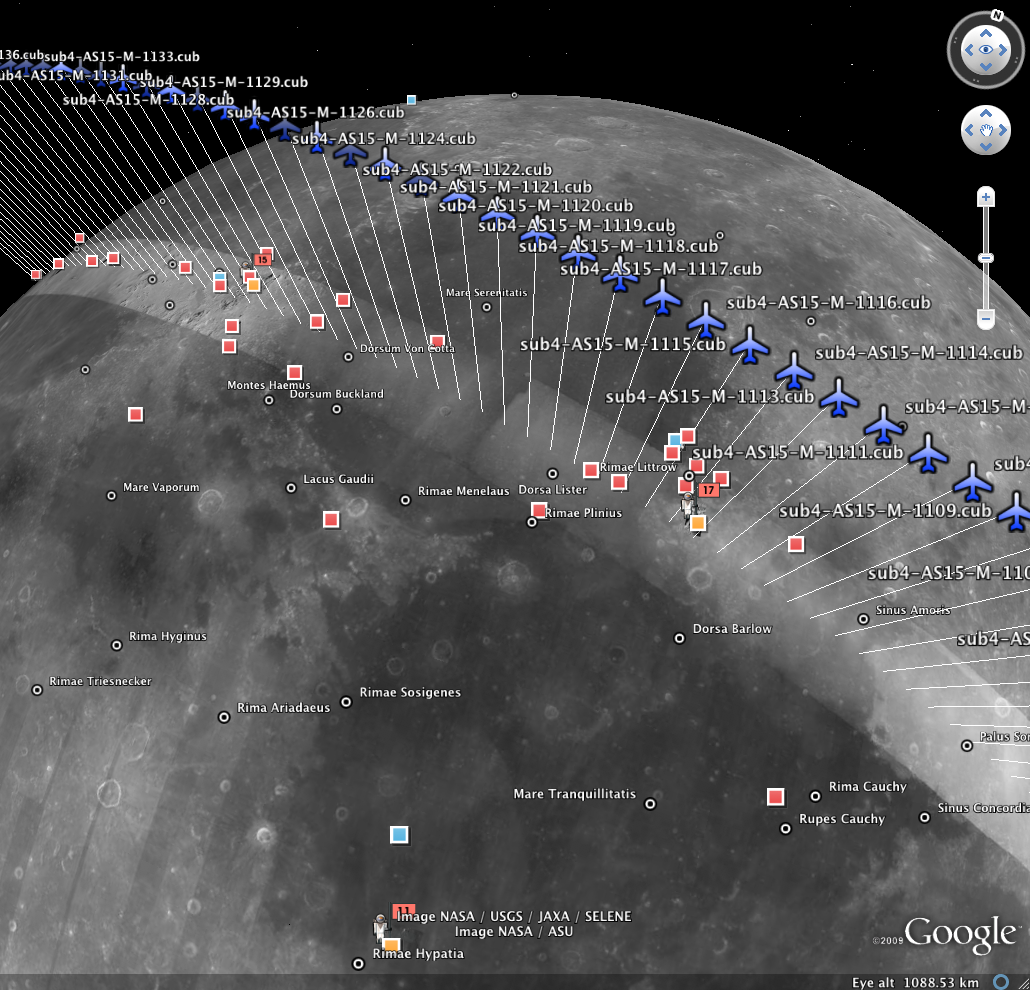
\includegraphics[width=6in]{images/orbitviz_ge_result.png}
  \end{center}
  \caption{ Example of a \ac{KML} visualization produced with {\tt
      orbitviz} depicting camera locations for the Apollo 15 Metric
    Camera during orbit 33 of the Apollo command module.}
  \label{fig:orbitviz_example}
\end{figure}

\begin{longtable}{|l|p{10cm}|}
\caption{Command-line options for orbitviz}
\label{tbl:orbitviz}
\endfirsthead
\endhead
\endfoot
\endlastfoot
\hline
Options & Description \\ \hline \hline
\texttt{--help|-h} & Display this help \\ \hline
\texttt{--output|-o \textit{filename(=orbit.kml)}} & Specifies the output file name \\ \hline
\texttt{--scale|-s \textit{float(=1)}} & Scale the size of the coordinate axes by this amount. Ex: To scale axis sizes up to earth size, use 3.66 \\ \hline
\texttt{--use-simple-placemarks} & Draw simple icons at camera locations, instead of a coordinate model \\ \hline
\end{longtable}


%--------------------------------------------------------------------------
%                       BUNDLE ADJUSTMENT TOOLS
%--------------------------------------------------------------------------

\section{isis\_adjust}

Bundle Adjustment for \ac{ISIS} images. This tool supports adjustment of
linescan cameras as well as simple frame cameras. For an in depth view
into how to use this tool, please read Chapter
\ref{ch:bundle_adjustment}.

\begin{longtable}{|l|p{10cm}|}
\caption{Command-line options for isis\_adjust}
\label{tbl:isise_adjust}
\endfirsthead
\endhead
\endfoot
\endlastfoot
\hline
Options & Description \\ \hline \hline
\texttt{--help|-h} & Display this help \\ \hline
\texttt{--cnet|-c \textit{control-network-file}} & Load a control network from a file \\ \hline
\texttt{--cost-function \textit{function(=L2)}} & Choose a robust cost function from \texttt{[L1|L2|Cauchy|Huber|PseudoHuberL1|L2|Cauchy|} \texttt{Huber|PseudoHuber]} \\ \hline
\texttt{--bundle-adjuster \textit{adjuster(=Sparse)}} & Choose a bundle adjustment version from \texttt{[Ref|Sparse|RobustRef|RobustSparse]} \\ \hline
\texttt{--disable-camera-const} & Disable the camera constraint error. This allows the cameras to move to pretty much anywhere. \\ \hline
\texttt{--disable-gcp-const} & Disable the GCP constraint error. \\ \hline
\texttt{--gcp-scalar \textit{multiplier(=1)}} & Sets a scalar to multiply to the sigmas (uncertainty) defined for the gcps. GCP sigmas are defined in the .gcp files. \\ \hline
\texttt{--lamda|-l \textit{float}} & Set the initial value of the LM paramater \texttt{g\_lambda}. If not set the algorithm will find the optimum starting point. \\ \hline
\texttt{--min-matches \textit{integer(=30)}} & Set the minimum number of matches between images that will be considered. \\ \hline
\texttt{--max-iterations \textit{integer(=25)}} & Set the maximum number of iterations \\ \hline
\texttt{--poly-order \textit{integer(=0)}} & Set the order of the polynomial used to adjust the camera properties. If using a frame camera, leave at 0 (meaning scalar offsets). For line scan cameras try 2. \\ \hline
\texttt{--position-sigma \textit{float(=100)}} & Set the sigma (uncertainty) of the spacecraft position. (meters) \\ \hline
\texttt{--pose-sigma \textit{float(=0.1)}} & Set the sigma (uncertainty) of the spacecraft pose. (radians) \\ \hline
\texttt{--report-level|-r \textit{integer(=10)}} & Changes the detail of the Bundle Adjustment Report. Valid values are 0 to 100 \\ \hline
\texttt{--robust-threshold \textit{float(=10)}} & Set the threshold for robust cost functions. \\ \hline
\texttt{--save-iteration-data|-s} & Saves all camera/point/pixel information between iterations for later viewing in \texttt{bundlevis} \\ \hline
\texttt{--seed-with-previous} & Use previous \texttt{isis\_adjust} files at starting for this run \\ \hline
\texttt{--write-isis-cnet-also} & Writes an ISIS style control network \\ \hline
\texttt{--write-kml [0|1(=0)]} & Selecting this will cause a KML file to be written with the GCPs. Set this flag to 1 and it will also write all the 3D position estimates of the points it is tracking in the KML. \\ \hline
\end{longtable}

%% \section{bundle\_adjust}
%% \label{bundle_adjust}

%% A generic bundle adjustment tool for ISIS images.  See Chapter
%% \ref{ch:bundle_adjustment} for more information.

%% \begin{longtable}{|l|p{10cm}|}
%% \caption{Command-line options for bundle\_adjust}
%% \label{tbl:bundle_adjust}
%% \endfirsthead
%% \endhead
%% \endfoot
%% \endlastfoot
%% \hline
%% Options & Description \\ \hline \hline
%% \verb#--help# & Display this table \\ \hline
%% \verb#-t arg(=isis)# & Select the stereo session type to use for processing. \\ \hline
%% \verb#-c arg# & Load a control network from a file. \\ \hline
%% \verb#-l arg# & Set the initial value of the LM parameter lambda \\ \hline
%% \verb#--robust-threshold arg (=10)# & Set the threshold for robust cost functions \\ \hline
%% \verb#-s# & Savae all camera information between iterations to iterCameraParam.txt, it also saves point locations for all iterations in iterPointsParam.txt \\ \hline
%% \verb# --min-matches arg (=30)# & When building a new control network, sets the minimum number of matches in a match to be added to the control network at a time. \\ \hline
%% \verb# -r arg (=10)# & Changes the detail of the Bundle Adjustment Report ( values range from 0 to 100 ). \\ \hline
%% \end{longtable}

\section{bundlevis}
\label{bundlevis}

The \texttt{bundlevis} program is a bundle adjustment result
visualizer.  See Chapter \ref{ch:bundle_adjustment} for more
information.

\begin{longtable}{|l|p{10cm}|}
\caption{Command-line options for bundlevis}
\label{tbl:bundlevis}
\endfirsthead
\endhead
\endfoot
\endlastfoot
\hline
Options & Description \\ \hline \hline
\texttt{--help|-h} & Display this help \\ \hline
\texttt{--camera-iteration-file|-c \textit{filename}} & Load the camera parameters for each iteration from this file \\ \hline
\texttt{--points-iteration-file|-p \textit{filename}} & Load the 3D points parameters for each iteration from this file \\ \hline
\texttt{--pixel-iteration-file|-x \textit{filename}} & Load pixel information data. Allowing for an illustration of the pixel data over time \\ \hline
\texttt{--control-network-file|-n \textit{filename}} & Load a control network for point and camera relationship status \\ \hline
\texttt{--additional-pnt-files \textit{filename(s)}} & Plot additional point files simultaneously with the above data \\ \hline
\texttt{--fullscreen} & Render with the entire screen \\ \hline
\texttt{--stereo} & Render in anagylph mode \\ \hline
\texttt{--show-moon} & Draw a wireframe moon \\ \hline
\texttt{--show-mars} & Draw a wireframe mars \\ \hline
\texttt{--show-earth} & Draw a wireframe earth \\ \hline
\end{longtable}


%% \section{reconstruct}
%% \label{reconstruct}

%% Tool under development

%% \section{results}
%% \label{results}

%% Tool under development

%% \section{rmax\_adjust}
%% \label{ramx_adjust}

%% Bundle Adjustment tool specifically for the Yamaha RMAX unmanned
%% aerial vehicle.


